\documentclass[12pt]{article}

\usepackage[utf8]{inputenc}
\usepackage{amsmath,amssymb,hyperref,array,xcolor,multicol,verbatim,mathpazo}
\usepackage[normalem]{ulem}
\usepackage[pdftex]{graphicx}
\usepackage{fullpage}

\usepackage{threeparttable}
\usepackage{geometry}
\usepackage[format=hang,font=normalsize,labelfont=bf]{caption}
\usepackage{lscape}
\usepackage{natbib}
\usepackage{setspace}
\usepackage{float,color}
\usepackage[pdftex]{graphicx}
\usepackage{pdfsync}
\usepackage{placeins}
\usepackage{geometry}
\usepackage{pdflscape}
\usepackage[normalem]{ulem}
\usepackage{threeparttable, multirow}
\useunder{\uline}{\ul}{}
\synctex=1
\usepackage{hyperref}
\hypersetup{colorlinks,linkcolor=red,urlcolor=blue,citecolor=blue}
\usepackage{bm}


\newcommand{\E}{\mathbb{E}}

% Identifying information
\title{
Homework 2
} 
\author{Linghui Wu}
\date{\today}

\begin{document}

\maketitle

\section{VARs}

\subsection*{Part (a)} 

Figure \ref{fig:time_series} represent the time series of Federal Funds Rate, the unemployment rate and the GDP deflator.

\begin{figure}[ht]
    \centering
    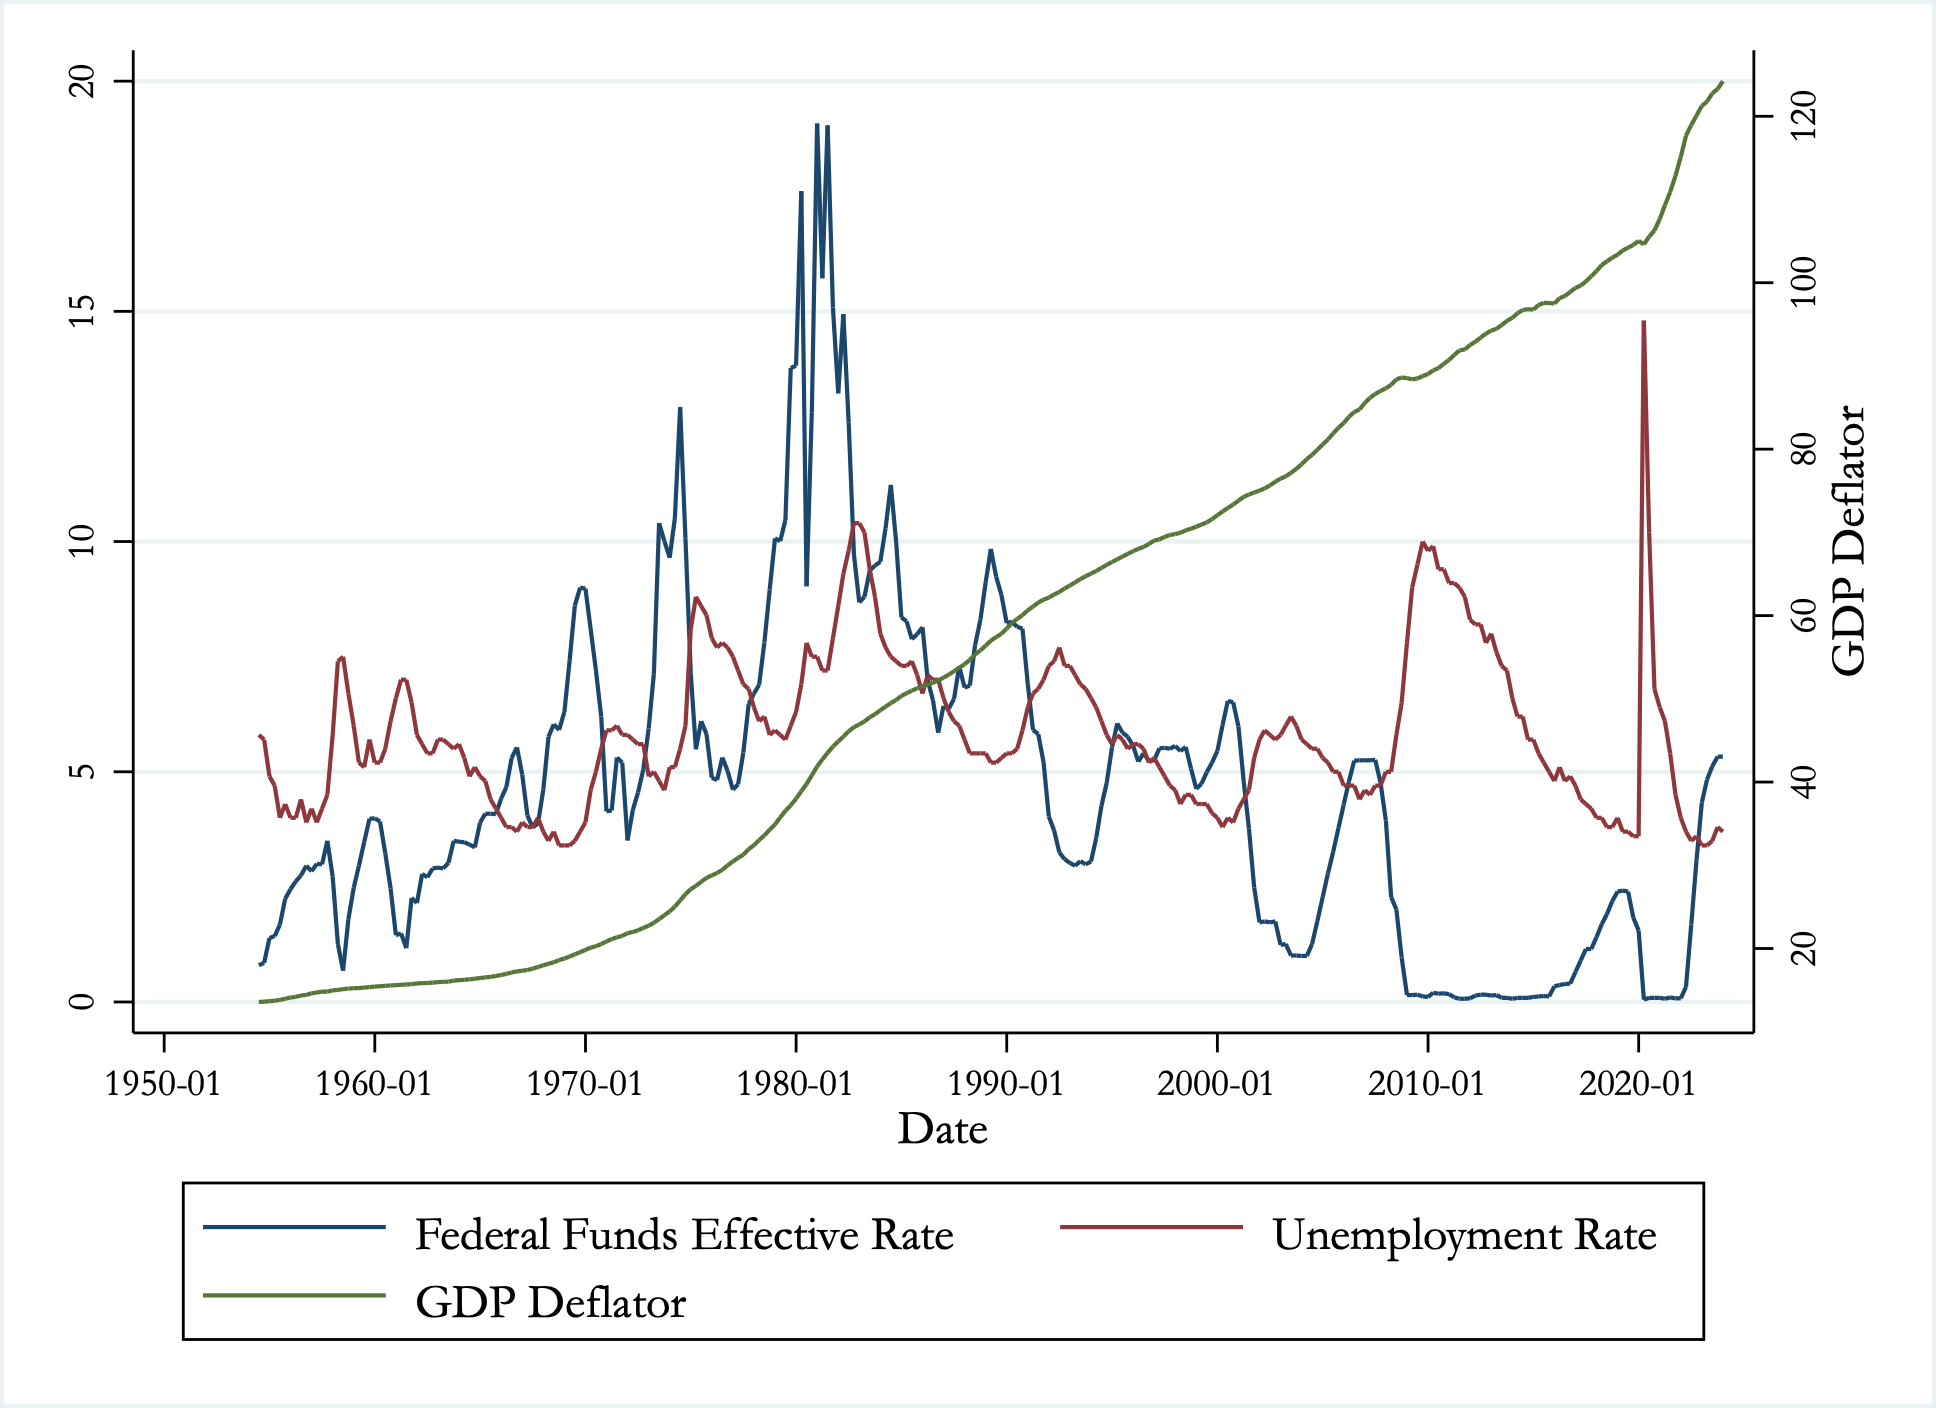
\includegraphics[width=0.8\textwidth]{figs/time_series.png}
    \caption{Federal Funds Rate, Unemployment and GDP Deflator}
    \label{fig:time_series}
\end{figure}

\subsection*{Part (c)} 

The sample period ends in 2007Q4 to exclude the potential impacts from the 2008 financial crisis. 
Specifially, the financial time series may become non-stationary after 2007Q4 due to structural changes in the data generating process.
Moreover, a VAR model would misinterpret the financial crisis as an internal monetary shock from the central bank. 

\subsection*{Part (d)} 

Figure \ref{fig:svar_irf} plot the impluse response functions from the SVAR.

\begin{figure}[ht]
    \centering
    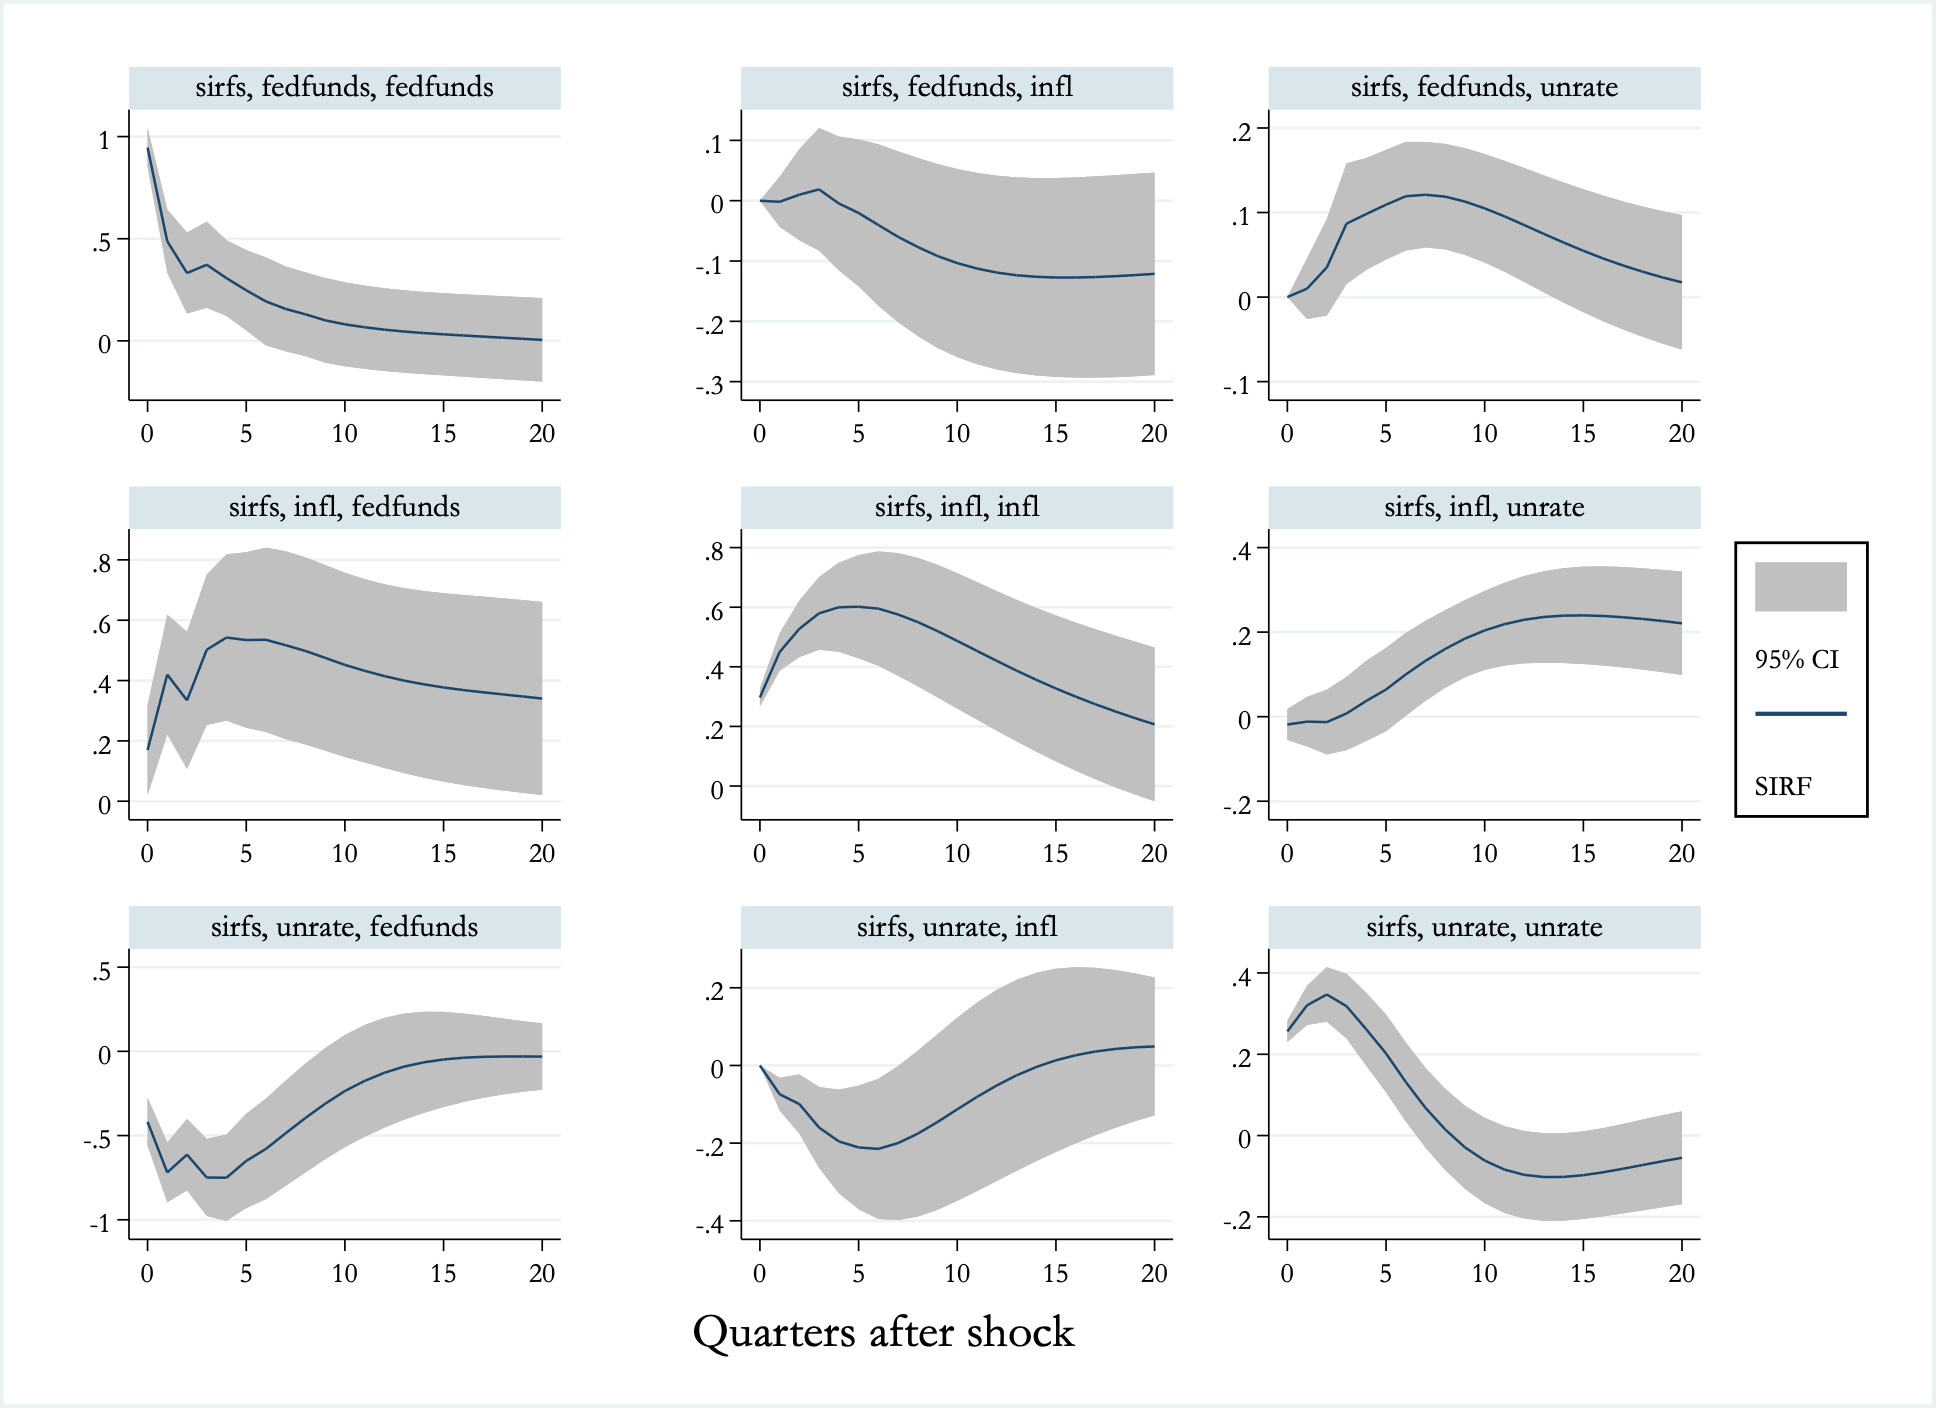
\includegraphics[width=0.8\textwidth]{figs/svar_irf.png}
    \caption{Impulse Response Functions}
    \label{fig:svar_irf}
\end{figure}

\subsection*{Part (e)} 

The interpretation of IRFs are as follows.

\begin{itemize}
    \item First Row: Following a shock to the Federal funds rate, inflation initially increases slightly before perrsistenly declining. 
    Unemployment first rises but eventually returns to the pre-shock level.

    \item Second Row: Given a shock to the inflation rate, the Federal funds rate gradually increases as the Fed reponds to the unexpected rise in inflation. 
    The Federal funds rate then tapers off, but remains above the pre-shock level. 
    The unemployment rate initially rises. 

    \item Third Row: An unemployment shock decreases initially the Federal funds rate and inflation. 
    In the long run, the shock's effects dissipate and both the Federal funds rate and the inflation return to their pre-shock levels.
\end{itemize}

\subsection*{Part (f)} 

Figure \ref{fig:estimated_shocks} exhibits the time series of the identified monetary shocks.

\begin{figure}[ht]
    \centering
    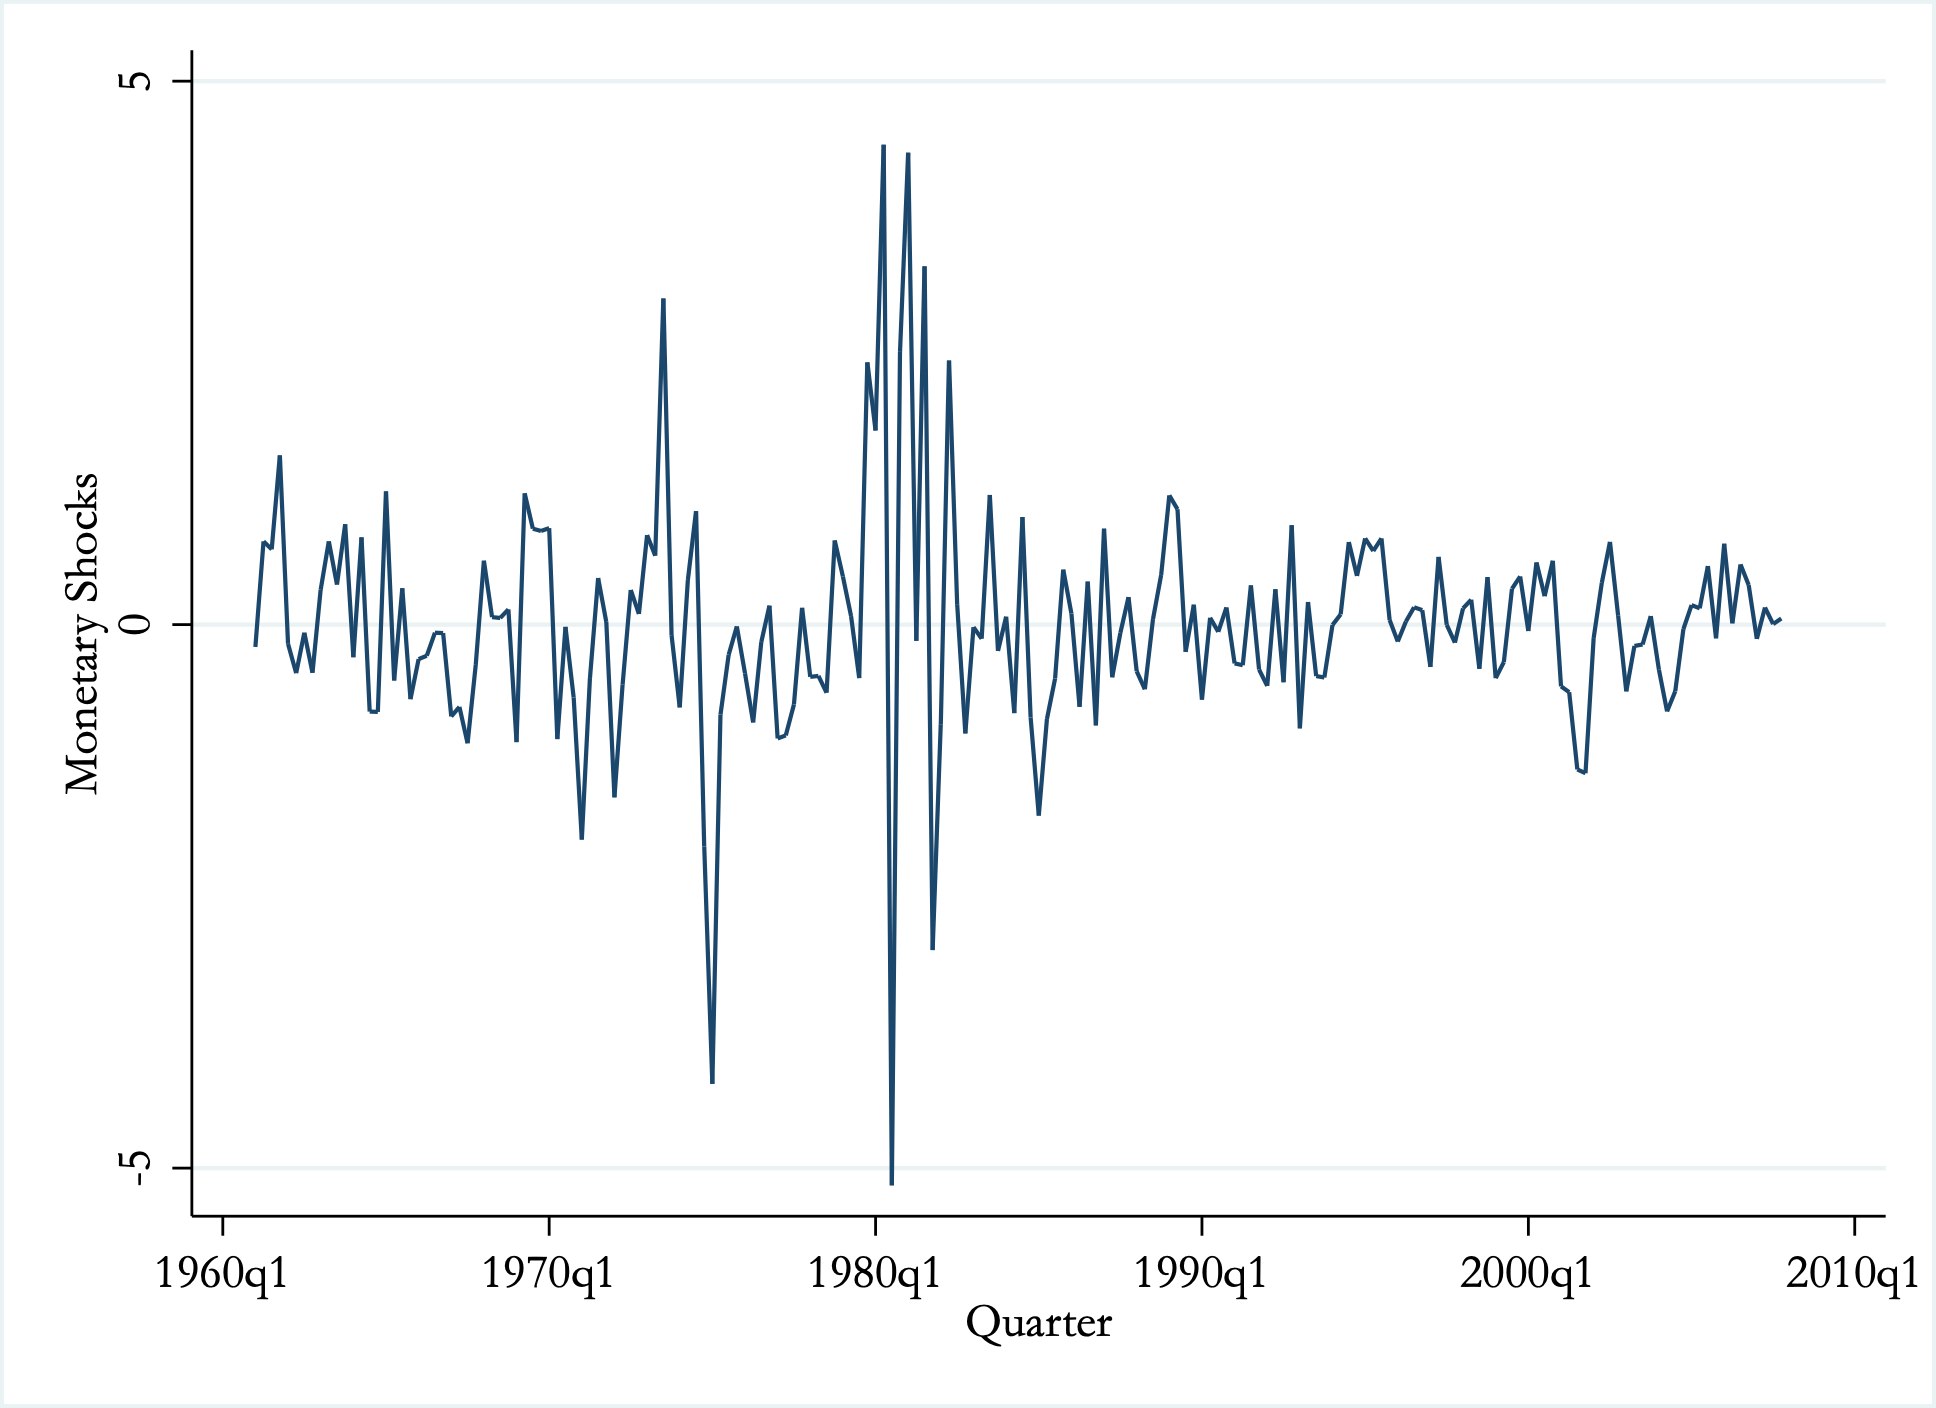
\includegraphics[width=0.8\textwidth]{figs/estimated_monetary_shocks}
    \caption{Identified Monetary Shocks}
    \label{fig:estimated_shocks}
\end{figure}


\subsection*{Part (g)} 

There are negative monetary shocks in 2001Q3 and 2001Q4, 
which correspond to the 9/11 terrorist attack. 
The Fed responded by lowering the interest rate to boost aggregate demand. 


\section{Romer Shocks}


\subsection*{Part (b)} 

Figure \ref{fig:var_irf_rr} shows the IRFs from the reduced-form VAR incorporating the Romer shocks.

\begin{figure}[ht]
    \centering
    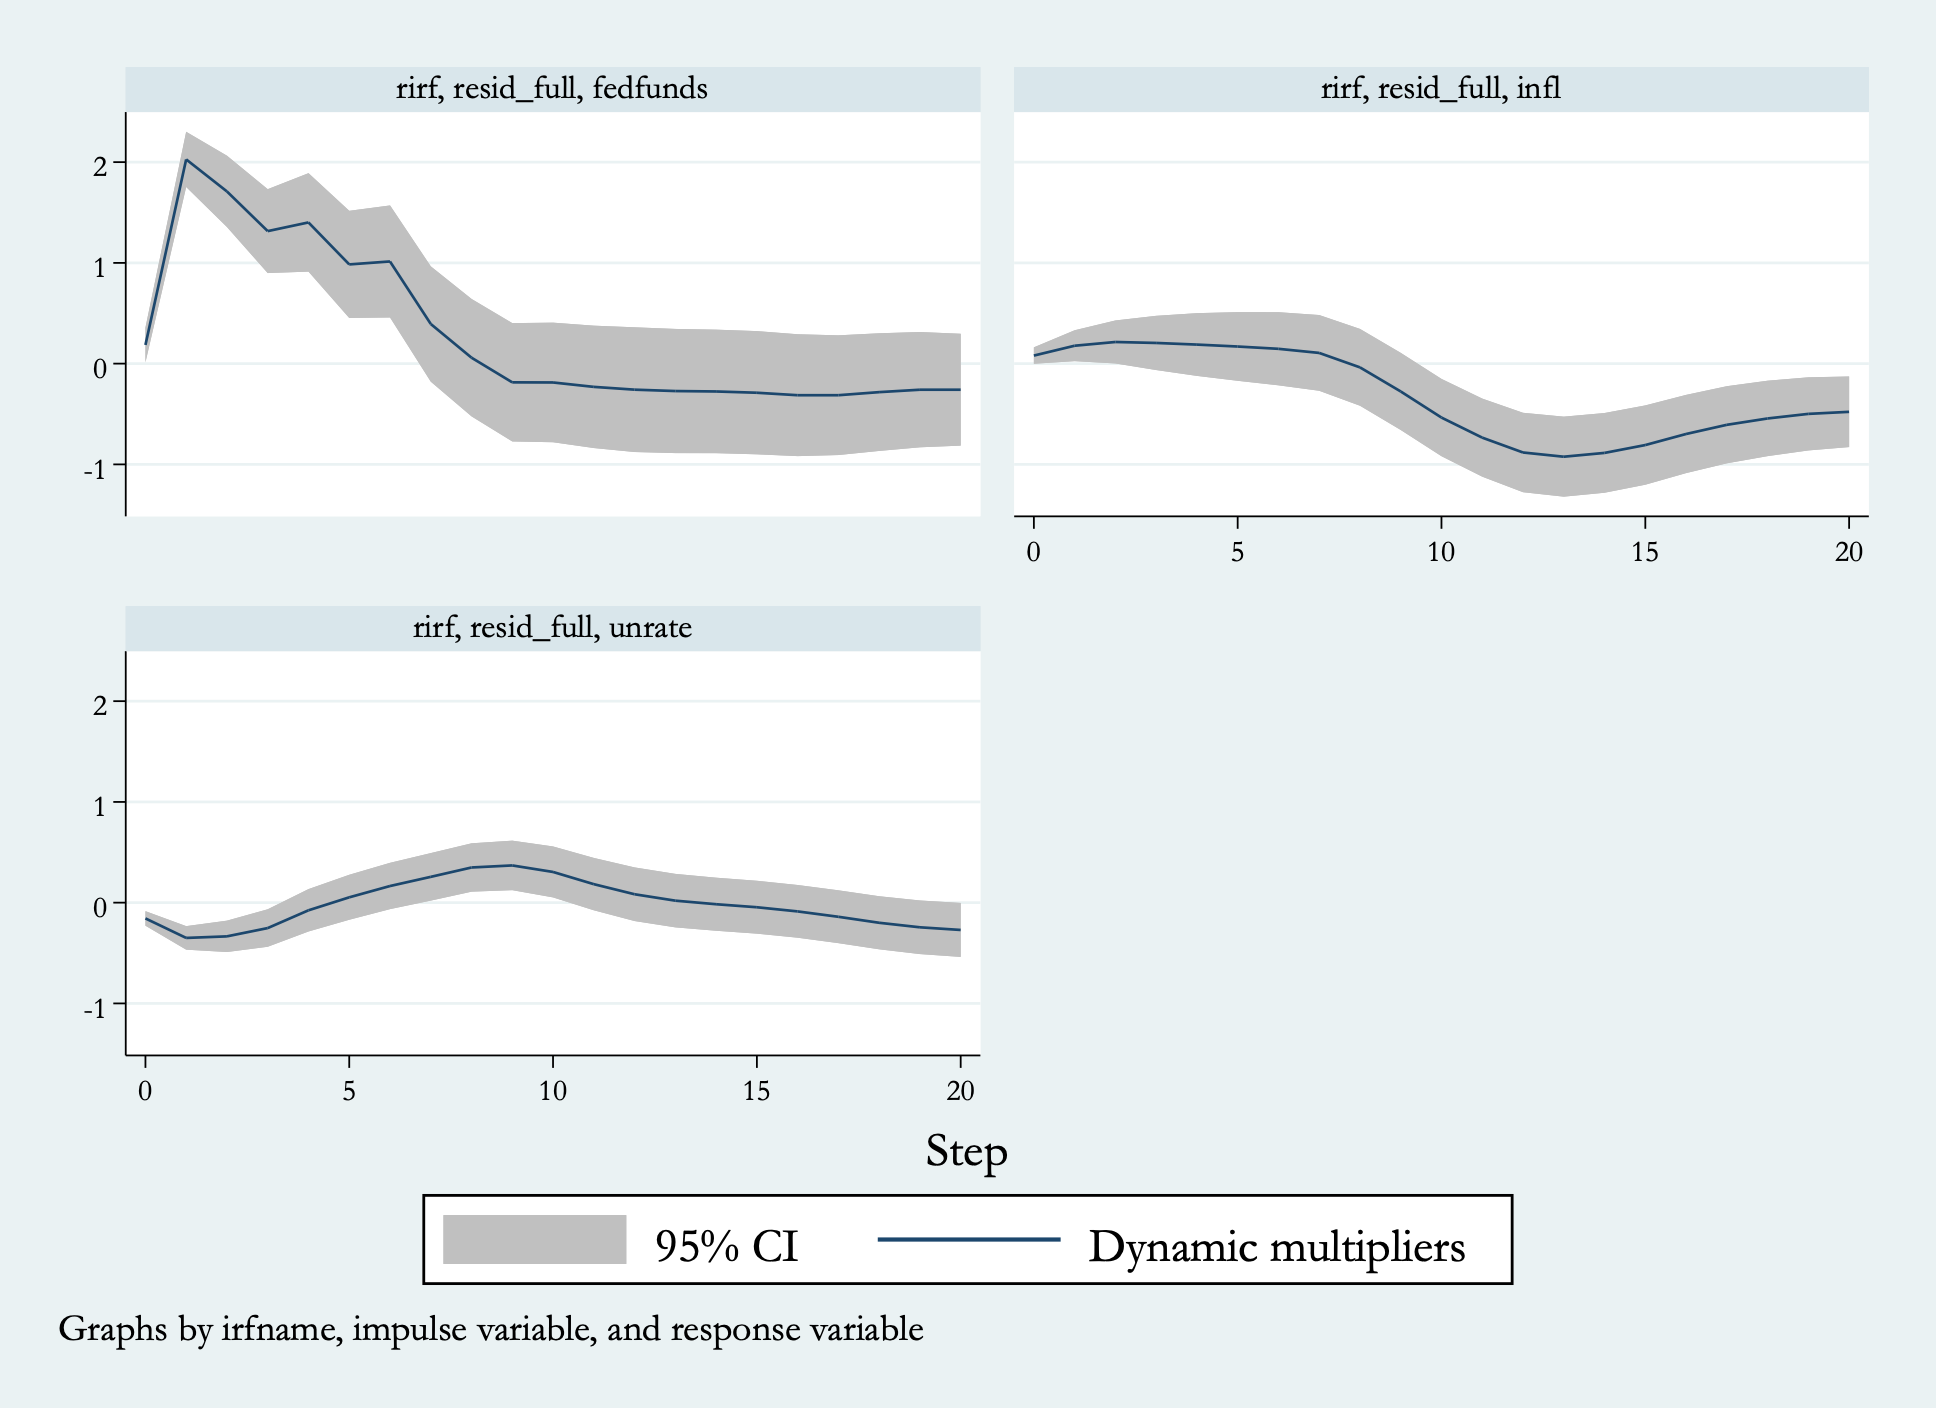
\includegraphics[width=0.8\textwidth]{figs/var_rirf.png}
    \caption{VAR Impulse Response Functions with Romer Shocks}
    \label{fig:var_irf_rr}
\end{figure}

\subsection*{Part (c)} 

Figure \ref{fig:svar_irf_rr} shows the IRFs from the structural VAR incorporating the Romer shocks.

\begin{figure}[ht]
    \centering
    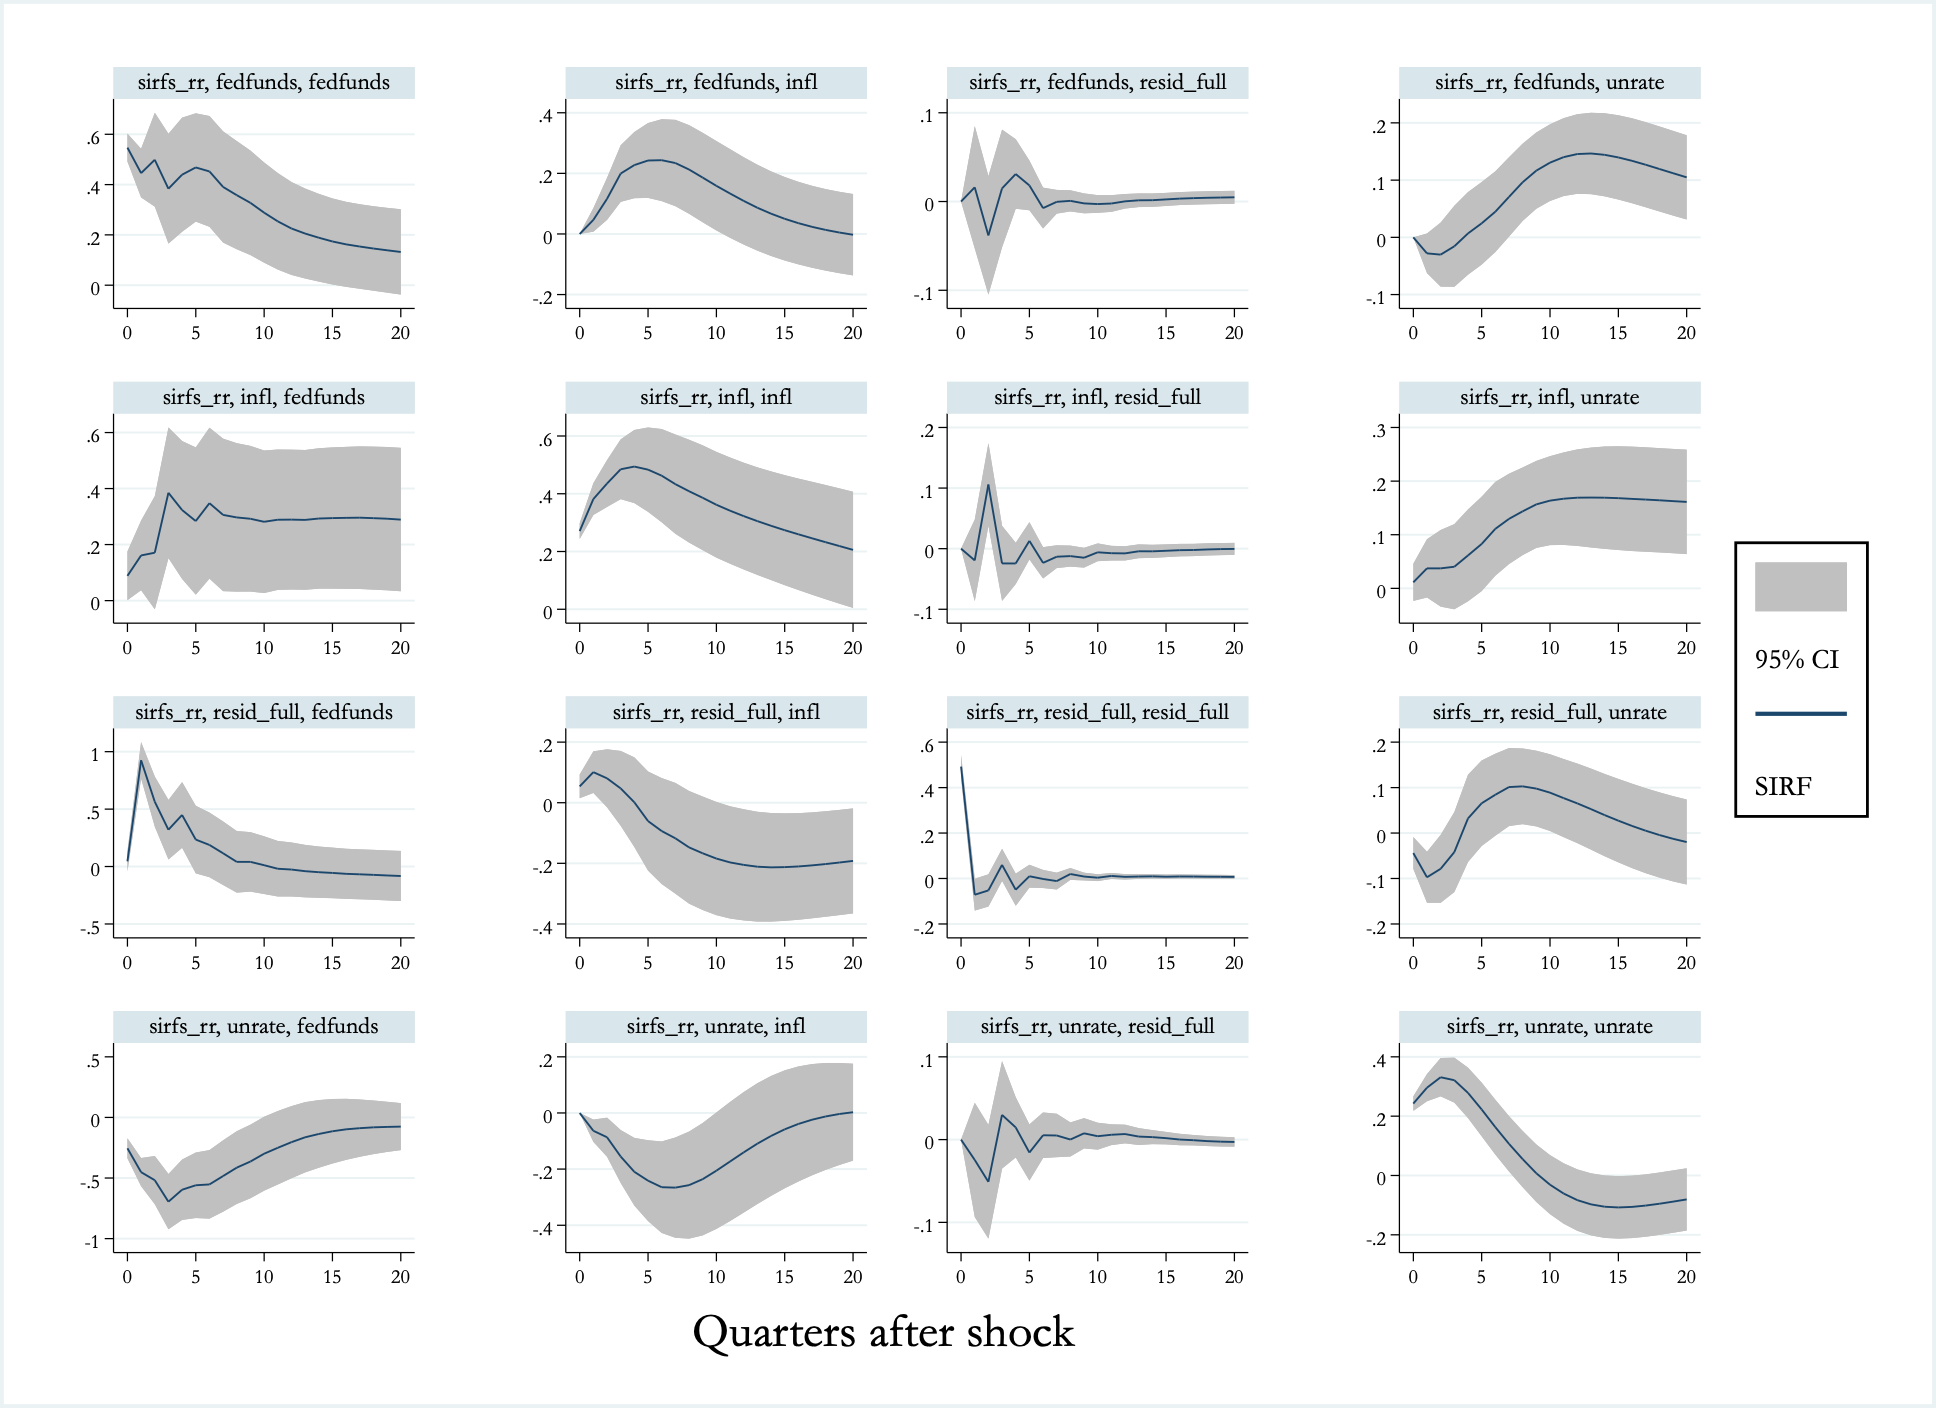
\includegraphics[width=0.8\textwidth]{figs/svar_irf_rr.png}
    \caption{SVAR Impulse Response Functions with Romer Shocks}
    \label{fig:svar_irf_rr}
\end{figure}

\subsection*{Part (d)} 

By ordering the Romer shocks first in the VAR, 
we impose the assumption that Romer shocks have a contemporaneous effect on the Federal funds rate, the inflation rate and the unemployment, but not vise versa. 
This is sensible because Romer and Romer (2004) argue that their shocks represent unanticipated movements in the monetary policy. 

\subsection*{Part (e)} 

Comparing figure \ref{fig:var_irf_rr} and figure \ref{fig:svar_irf_rr}, 
we observe the estimated dynamic effects from Romer shocks on other financial variables are relatively larger and less responsive in reduced-form VARs. 

This can be explained by the fact that, in SVAR, 
the unemployment is influenced by the contemporaneous inflation and the Romer shocks plus the lagged terms. 
While in the reduced-form VAR, we include Romer shocks as control variables,
thereby shutting down the contemporaneous effects from inflation and Romer shocks. 

\subsection*{Part (f)} 

Comparing figure \ref{fig:svar_irf} and figure \ref{fig:svar_irf_rr}, 
we see the dynamic effect of the Federal funds rate on the inflation becomes more apparent. Following a Romer shock, the inflation decreases with a greater magnitude. 
It is likely that a non-Romer monetary shock incorporates some endogeneity that is positively correlated with inflation, 
along with anticipation effects reflecting the Fed's preemptive actions to inflation. 
With Romer monetary shocks, we obtained a ``cleaner'' estimated effects of monetary policy. 

\subsection*{Part (g)} 

Figure \ref{fig:compare_shocks} compares the Romer monetary shocks and the SVAR-identified monetary shocks. 
Overall, Romer monetary shocks exhibits a less fluctuating pattern. 
During the 2001Q3 and 2001Q4 period, the effect of negative monetary shock still presents but is much smaller in contrast to the SVAR-identified shocks.

\begin{figure}[ht]
    \centering
    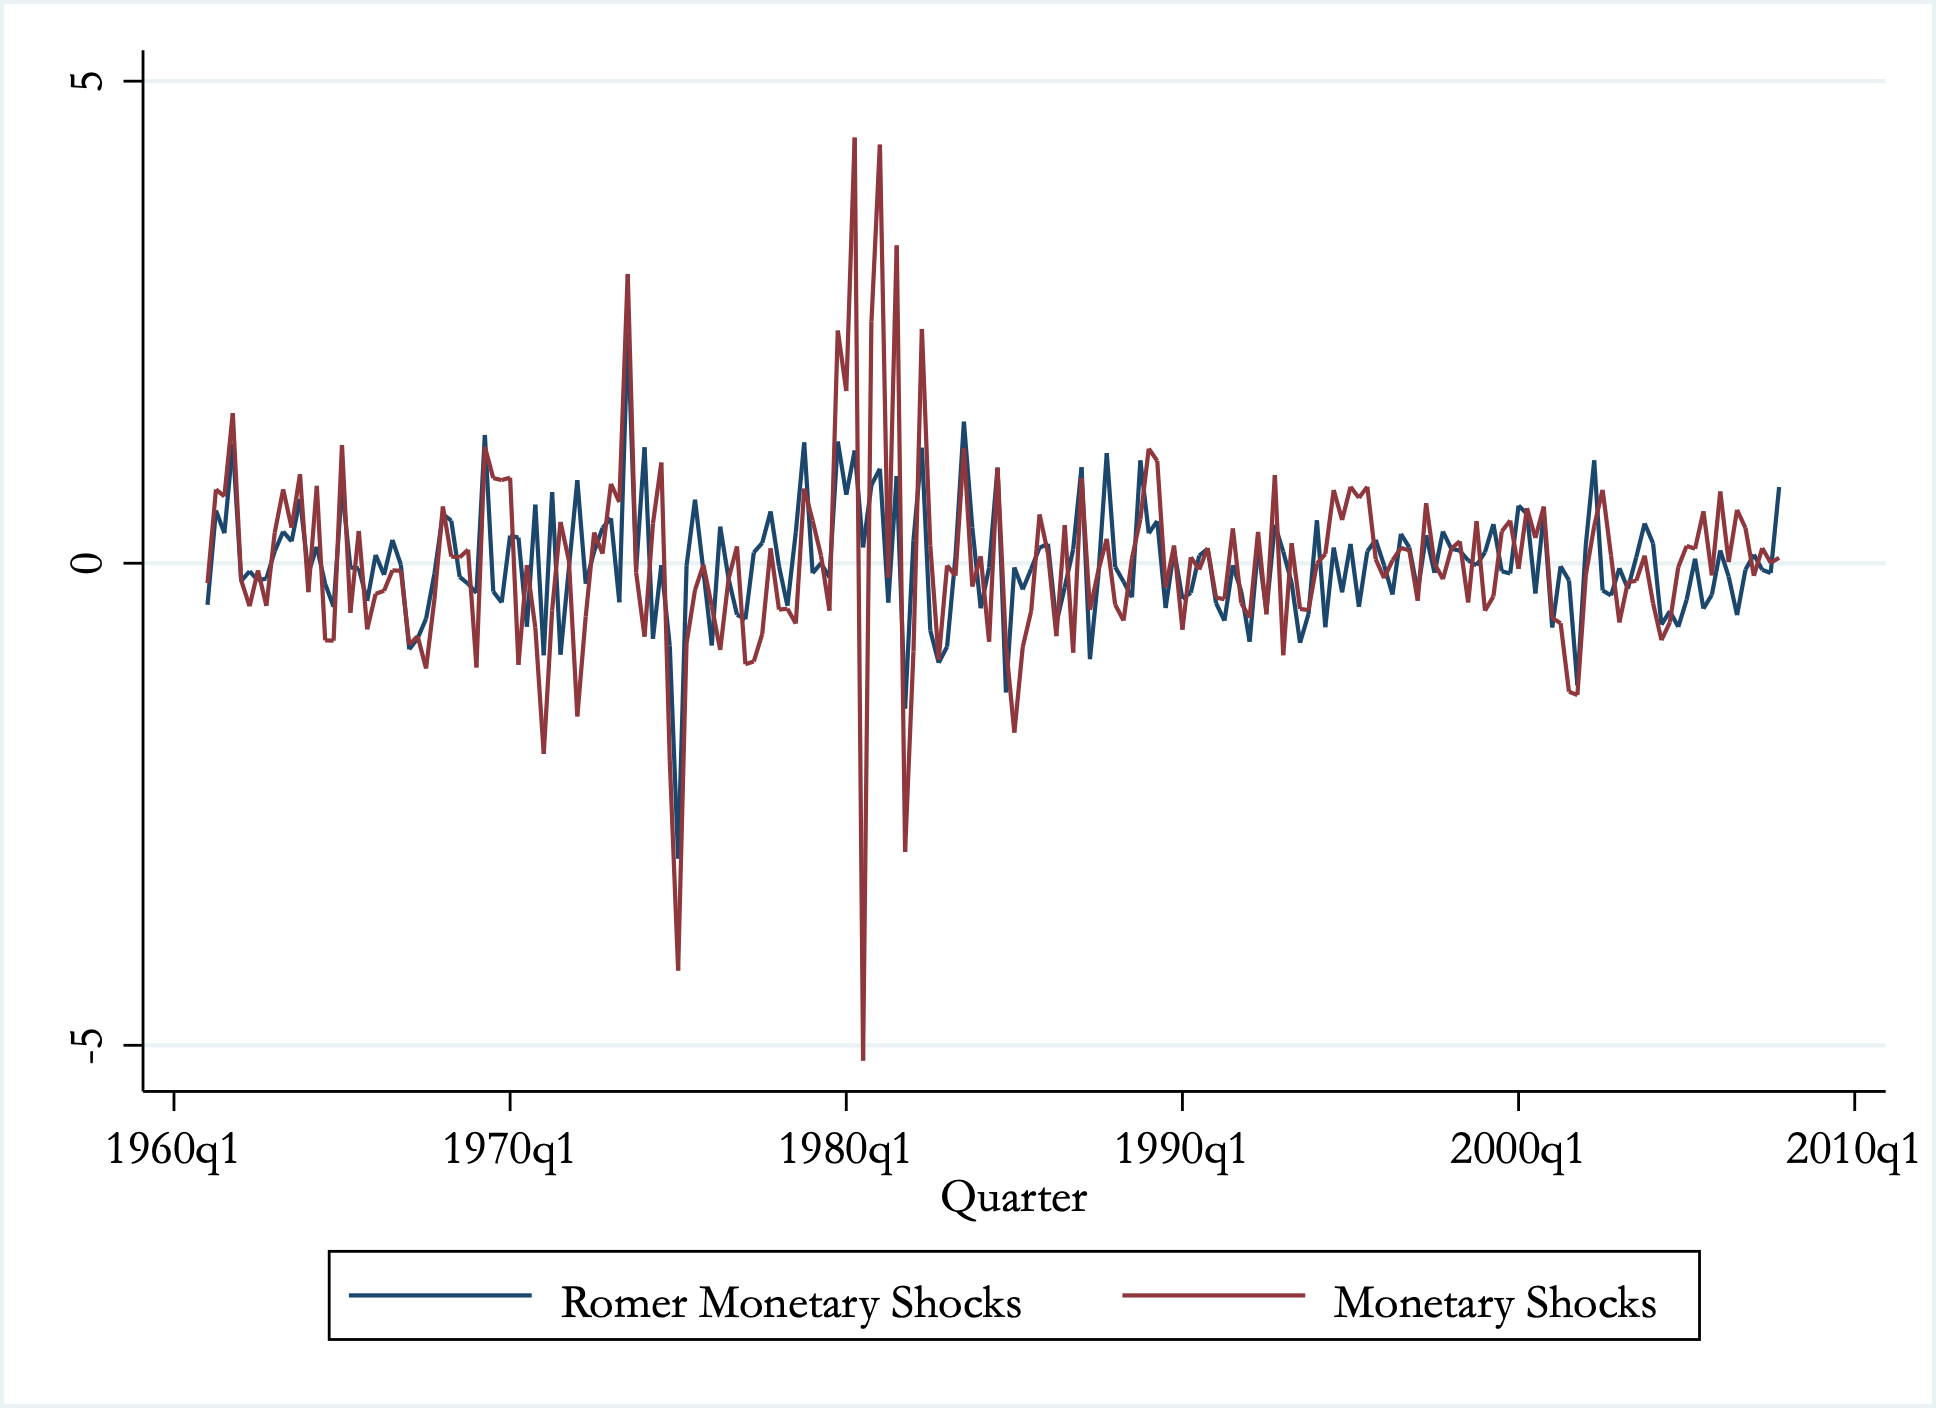
\includegraphics[width=0.8\textwidth]{figs/compare_monetary_shocks}
    \caption{Comparison of Romer and SVAR-Identified Monetary Shocks}
    \label{fig:compare_shocks}
\end{figure}


\end{document}


